\documentclass{beamer}

%\usepackage[magyar]{babel}
\usepackage[utf8]{inputenc}
\usepackage{graphicx}
%\setbeamersize{text margin left=10pt,text margin right=5pt}

\usetheme{Antibes}
\usecolortheme[RGB={255,50,50}]{structure}

\author{D. G. O.}
\title{Kvantum titkosítás}
\subtitle{Modern fizikai kísérletek szeminárium\\2015-2016 tavaszi félév}
\institute{Eötvös Loránd Tudományegyetem}
\date{2016. március 11.}

\begin{document}

    \small

    \begin{frame}
        \titlepage
    \end{frame}

    \section{Tartalom}

    \begin{frame}

        \center

        \textbf{Tartalom}

        \begin{itemize}
            \item Klasszikus titkosítás
            \begin{itemize}
                \item Egyszerű módszerek
                \item Problémái
            \end{itemize}
            \item Kvantummechanika, elméleti bevezetés
            \item Quantum Key Distribution protokolok
            \begin{itemize}
                \item Határozatlansági elven alapuló
                \item Kvantum összefonódáson alapuló
            \end{itemize}
            \item Kísérletek, gyakorlati megvalósítások
            \item Felhasználás, példák
        \end{itemize}
    \end{frame}

    \section{Bevezetés}

    \begin{frame}

        \center

        \textbf{Szimmetrikus titkosítás}

        \hspace{5pt}

        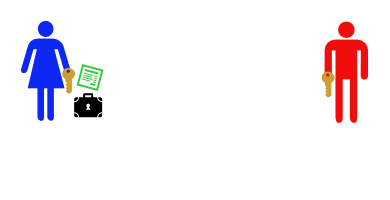
\includegraphics[trim={0 50px 0 15px},clip,width=0.4\textwidth]{shared1.png}\\
        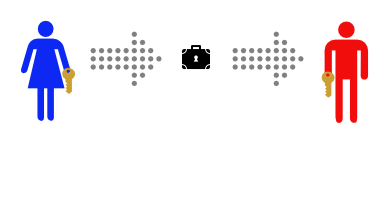
\includegraphics[trim={0 50px 0 15px},clip,width=0.4\textwidth]{shared2.png}\\
        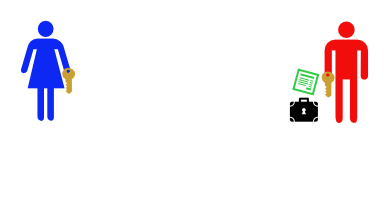
\includegraphics[trim={0 50px 0 15px},clip,width=0.4\textwidth]{shared3.png}

        \begin{itemize}
            \item Alice (A) és Bob (B) ismeri a kulcsot.
            \item Ugyanazzal a kulccsal titkosítják és fejtik meg az üzenetet.
            \item Probléma: Hogyan tudatják egymással mi a titkos kulcs?
        \end{itemize}

    \end{frame}

    \begin{frame}

        \center

        \textbf{Aszimmetrikus titkosítás}

        \hspace{5pt}

        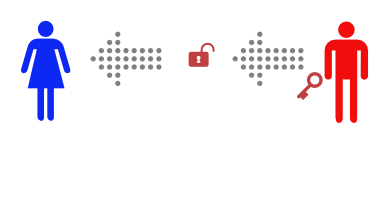
\includegraphics[trim={0 50px 0 15px},clip,width=0.4\textwidth]{public2.png}\\
        
\includegraphics[trim={0 50px 0 15px},clip,width=0.4\textwidth]{public3.png}\\
        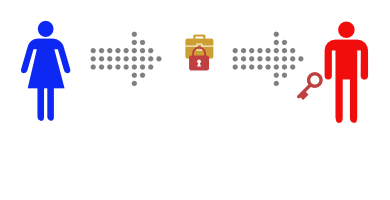
\includegraphics[trim={0 50px 0 15px},clip,width=0.4\textwidth]{public4.png}

        \begin{itemize}
            \item Bob csak a publikus kulcsot küldi el, a privát kulcs nála marad.
            \item Szétoszthatják egymás között a szimmetrikus kulcsot.
        \end{itemize}

    \end{frame}

    \section{Klasszikus kriptigráfia}

    \begin{frame}

        \center

        \textbf{Klasszikus public key distribution}

        \begin{itemize}
            \item Determinisztikus algoritmussal a nyílt kulcs kódolja az üzenetet.
            \item Egy \textbf{gyakorlatilag} kivitelezhetetlen algoritmus tudná visszafejteni.
            \item Titkos kulccsal egyszerű a visszafejtés.
            \item Két fő csoport:
                \begin{itemize}
                    \item Prímfelbontáson alapuló
                    \item Diszkrét logaritmus eljáráson alapuló
                \end{itemize}
        \end{itemize}

    \end{frame}

    \subsection{Prímfelbontáson alapuló eljárások}

    \begin{frame}

        \center

        \textbf{Prímfelbontáson alapuló eljárások problémája}

        \begin{itemize}
            \item RSA algoritmus vázlata:
                \begin{enumerate}
                    \item Generálunk $p$, $q$ prímszámokat.
                    \item Publikus kulcs egyik eleme: $n = p \cdot q$.
                    \item Titkos kulcs: $d = (p - 1) \cdot (q - 1)$.
                \end{enumerate}
            \item Felbontva $n$-t kitalálható $d$ a titkos kulcs.
            \item 2009 december: RSA-768 (kb. 768 bites publikus kulcs) faktorizációja:
                \begin{itemize}
                    \item 2 évig tartott.
                    \item Megfelel 2000 évnyi számolásnak 2.2 GHz-es AMD Opteron processzoron.
                \end{itemize}
            \item 2016-ban ajánlott legalább 2048 bites kulcs.
        \end{itemize}

    \end{frame}

    \begin{frame}

        \center

        \textbf{Prímfelbontáson alapuló eljárások problémája}

        \begin{itemize}
            \item Problémák:
                \begin{itemize}
                    \item Mai legjobb prímfelbontó algoritmusok futásideje szám nagyságával exponenciálisan növekednek, de\\
                    nem bizonyított, hogy nincs \textit{elég gyors} algoritmus a prímfelbontásra.
                    \item Mindig növelni kell a kulcs méretét
                    \item Kvantumszámítógépekkel lehet polinomiális időben felbontani prímet.\\
                        Eddigi legnagyobb prím, amit faktorizáltak, 2012-ben 56153.
                    \item Kvantumszámítógépek ha elterjednek, klasszikus algoritmusok könnyen feltörhetőek.
                    \item (Hasonló problémák más klasszikus aszimmetrikus kriptográfiára.)
                \end{itemize}
        \end{itemize}

    \end{frame}

    \section{Kvantum kriptográfia alapjai}

    \begin{frame}

        \center

        \textbf{Kvantumkriptográfia alapjai}

        \hspace{5pt}

        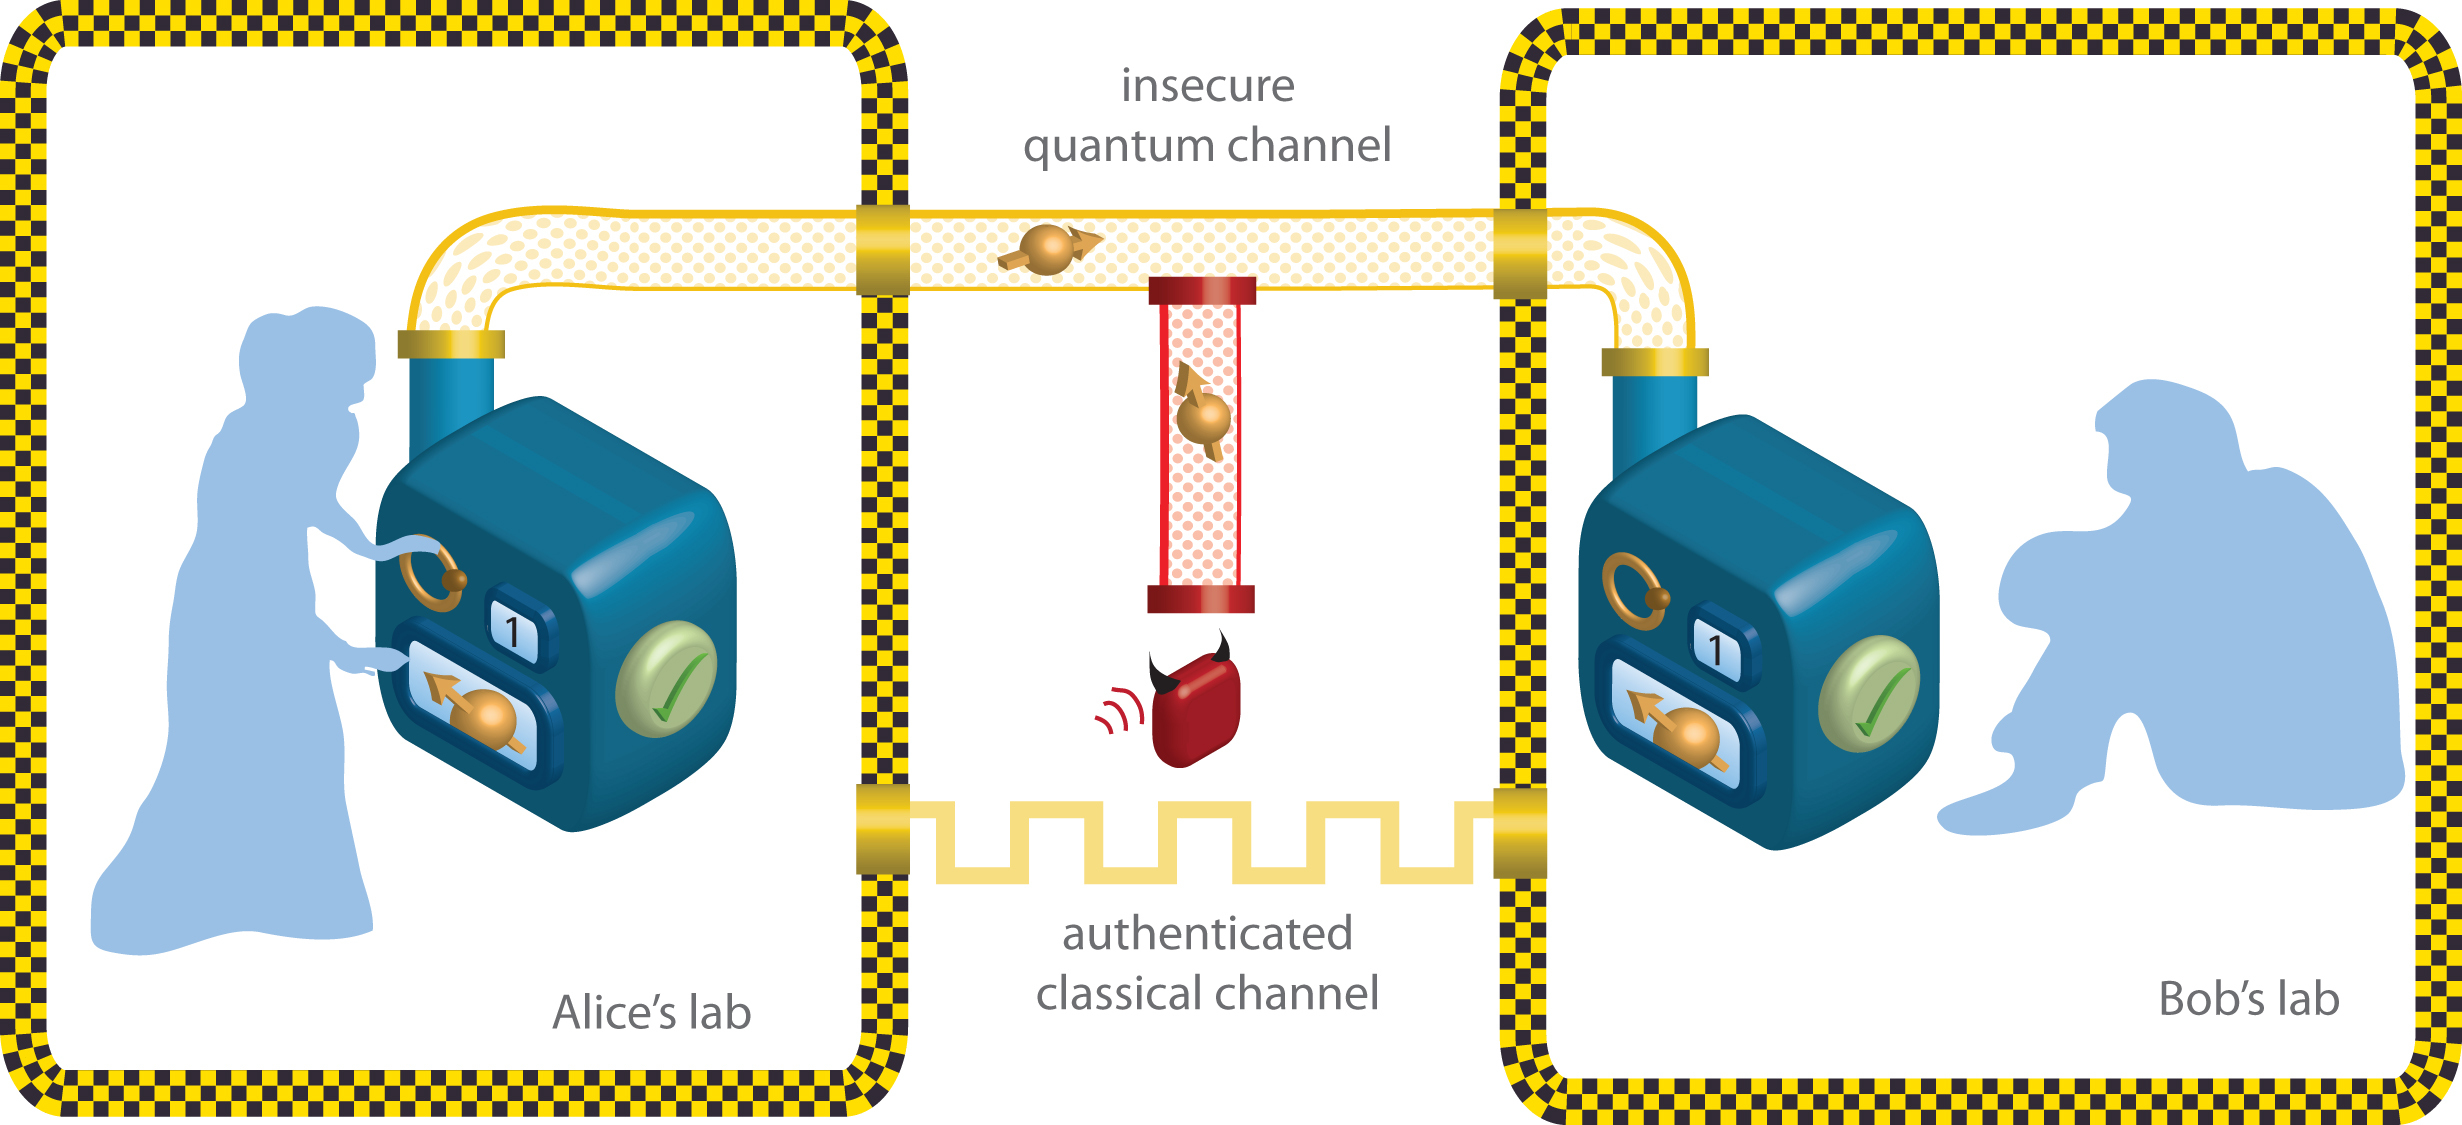
\includegraphics[width=0.9\textwidth]{quantum_alice_and_bob.jpg}

        \begin{itemize}
            \item Kvantumos csatornán osztják meg a kulcsot.
            \item Kvantumállapotot osztanak meg.
            \item Például egy foton, aminek a spinje az információ.
        \end{itemize}

    \end{frame}

    \subsection{Határozatlansági elven alapuló eljárások}

    \begin{frame}

        \center

        \textbf{Határozatlansági elven alapuló eljárások}

        \begin{itemize}
            \item Eljárás vázlata:
            \begin{itemize}
                \item Kulcsot szeretnénk generálni, amit csak Alice és Bob ismerhet.
                \item A teljes kulcs: bitek, fotonok mérésének eredménye.
                \item Alice polarizált fotonokat küld véletlenszerű bázisokban.\\
                    $\left| \psi_1 \right\rangle, \left| \psi_2 \right\rangle, \left| \psi_3 \right\rangle, ...$
                \item Bob méri a fotonokat véletlenszerű bázisokban.
                \item Összes mérés után kijelentik milyen bázisokban mértek.
                \item Ahol a bázisaik megegyeztek, azokból áll a kulcsuk.
            \end{itemize}
        \end{itemize}

    \end{frame}

    \begin{frame}

        \center

        \textbf{BB84 protokol}

        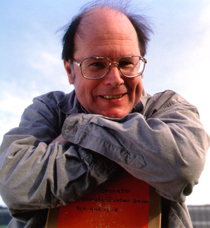
\includegraphics[height=100pt]{bennett.jpg}
        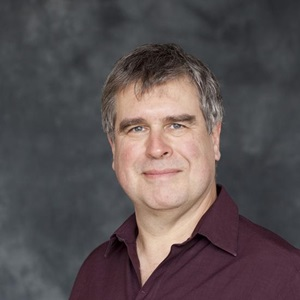
\includegraphics[height=100pt]{brassard.jpg}

        \begin{itemize}
            \item Charles Bennett, Gilles Brassard, 1984
            \item Első kvantumtitkosítási protokol
        \end{itemize}

    \end{frame}

    \begin{frame}

        \center

        \textbf{BB84 protokol}

        \begin{itemize}
            \item Alice polarizált fotonokat küld.
            \item 2 féle bázisban kódolhatja 1-et és 0-t.
                \begin{itemize}
                    \item ($+$) bázis:
                        \begin{itemize}
                            \item 0: $\left| \rightarrow \right\rangle$
                            \item 1: $\left| \uparrow \right\rangle$
                        \end{itemize}
                    \item ($\times$) bázis:
                        \begin{itemize}
                            \item 0: $\left| \nearrow \right\rangle = \frac{1}{\sqrt{2}} \left( \left| \uparrow \right\rangle + \left| \rightarrow \right\rangle \right)$
                            \item 1: $\left| \nwarrow \right\rangle = \frac{1}{\sqrt{2}} \left( \left| \uparrow \right\rangle - \left| \rightarrow \right\rangle \right)$
                        \end{itemize}
                \end{itemize}
            \item Alice 4 állapotból összerakott sorozatot küld, pl.
        \end{itemize}

        \begin{tabular}{|c|c|c|c|c|c|c|c|c|}
            \hline
            Választott bázis
            & $+$
            & $+$
            & $\times$
            & $+$
            & $\times$
            & $\times$
            & $\times$
            & $+$\\
            \hline
            Küldött foton
            & $\uparrow$
            & $\rightarrow$
            & $\nwarrow$
            & $\uparrow$
            & $\nwarrow$
            & $\nearrow$
            & $\nearrow$
            & $\rightarrow$\\
            \hline
            Küldött bit
            & 1
            & 0
            & 1
            & 1
            & 1
            & 0
            & 0
            & 0\\
            \hline
        \end{tabular}

    \end{frame}

    \begin{frame}

        \center

        \textbf{BB84 protokol}

        \begin{itemize}
            \item Alice küld egy $\left| \psi \right\rangle$ állapotot.
            \item Bob 2 db mérőműszere:
                \begin{itemize}
                    \item $\hat{P}_+ = \left| \uparrow \right\rangle \left\langle \uparrow \right|$
                        \begin{itemize}
                            \item Ha $\left| \psi \right\rangle = \left| \rightarrow \right\rangle$, akkor 0-t mér (nincs beütés a fotonszámlálón)
                            \item Ha $\left| \psi \right\rangle = \left| \uparrow \right\rangle$, akkor 1-t mér (van beütés a fotonszámlálón)
                            \item Ha $\left| \psi \right\rangle = \left| \nearrow \right\rangle$ vagy $\left| \nwarrow \right\rangle$ akkor 0-t vagy 1-t mér 50 \% valószínűséggel.
                        \end{itemize}
                    \item $\hat{P}_\times = \left| \nwarrow \right\rangle \left\langle \nwarrow \right|$
                        \begin{itemize}
                            \item Ha $\left| \psi \right\rangle = \left| \nearrow \right\rangle$, akkor 0-t mér (nincs beütés a fotonszámlálón)
                            \item Ha $\left| \psi \right\rangle = \left| \nwarrow \right\rangle$, akkor 1-t mér (van beütés a fotonszámlálón)
                            \item Ha $\left| \psi \right\rangle = \left| \rightarrow \right\rangle$ vagy $\left| \uparrow \right\rangle$ akkor 0-t vagy 1-t mér 50 \% valószínűséggel.
                        \end{itemize}
                \end{itemize}
        \end{itemize}

    \end{frame} 

    \begin{frame}

        \center

        \textbf{BB84 protokol}

        \begin{itemize}
            \item Példa
        \end{itemize}

        \footnotesize

        \begin{tabular}{|c|c|c|c|c|c|c|c|c|}
            \hline
            Alice bázisa
            & $+$
            & $+$
            & $\times$
            & $+$
            & $\times$
            & $\times$
            & $\times$
            & $+$\\
            \hline
            Küldött foton
            & $\uparrow$
            & $\rightarrow$
            & $\nwarrow$
            & $\uparrow$
            & $\nwarrow$
            & $\nearrow$
            & $\nearrow$
            & $\rightarrow$\\
            \hline
            Bob bázisa
            & $+$
            & $\times$
            & $\times$
            & $\times$
            & $+$
            & $\times$
            & $+$
            & $+$\\
            \hline
            Bob mért értéke
            & 1
            & 
            & 1
            & 
            & 
            & 0
            & 
            & 0\\
            \hline
        \end{tabular}

        \begin{itemize}
            \item Alice és Bob nyílvánosan megosztja bázisait ezután.
            \item Ahol bázisaik megegyeznek, ott ugyanaz az érték.
            \item Az értékeket senki más nem tudhatja, csak a bázist.
            \item Ahol bázisaik megegyeznek, az lesz a kulcs!
            \item Titkos kulcs: 1100
        \end{itemize}

    \end{frame}

    \begin{frame}

        \center

        \textbf{BB84 protokol}

        \begin{itemize}
            \item Lehallgathatja-e valaki őket?
        \end{itemize}

        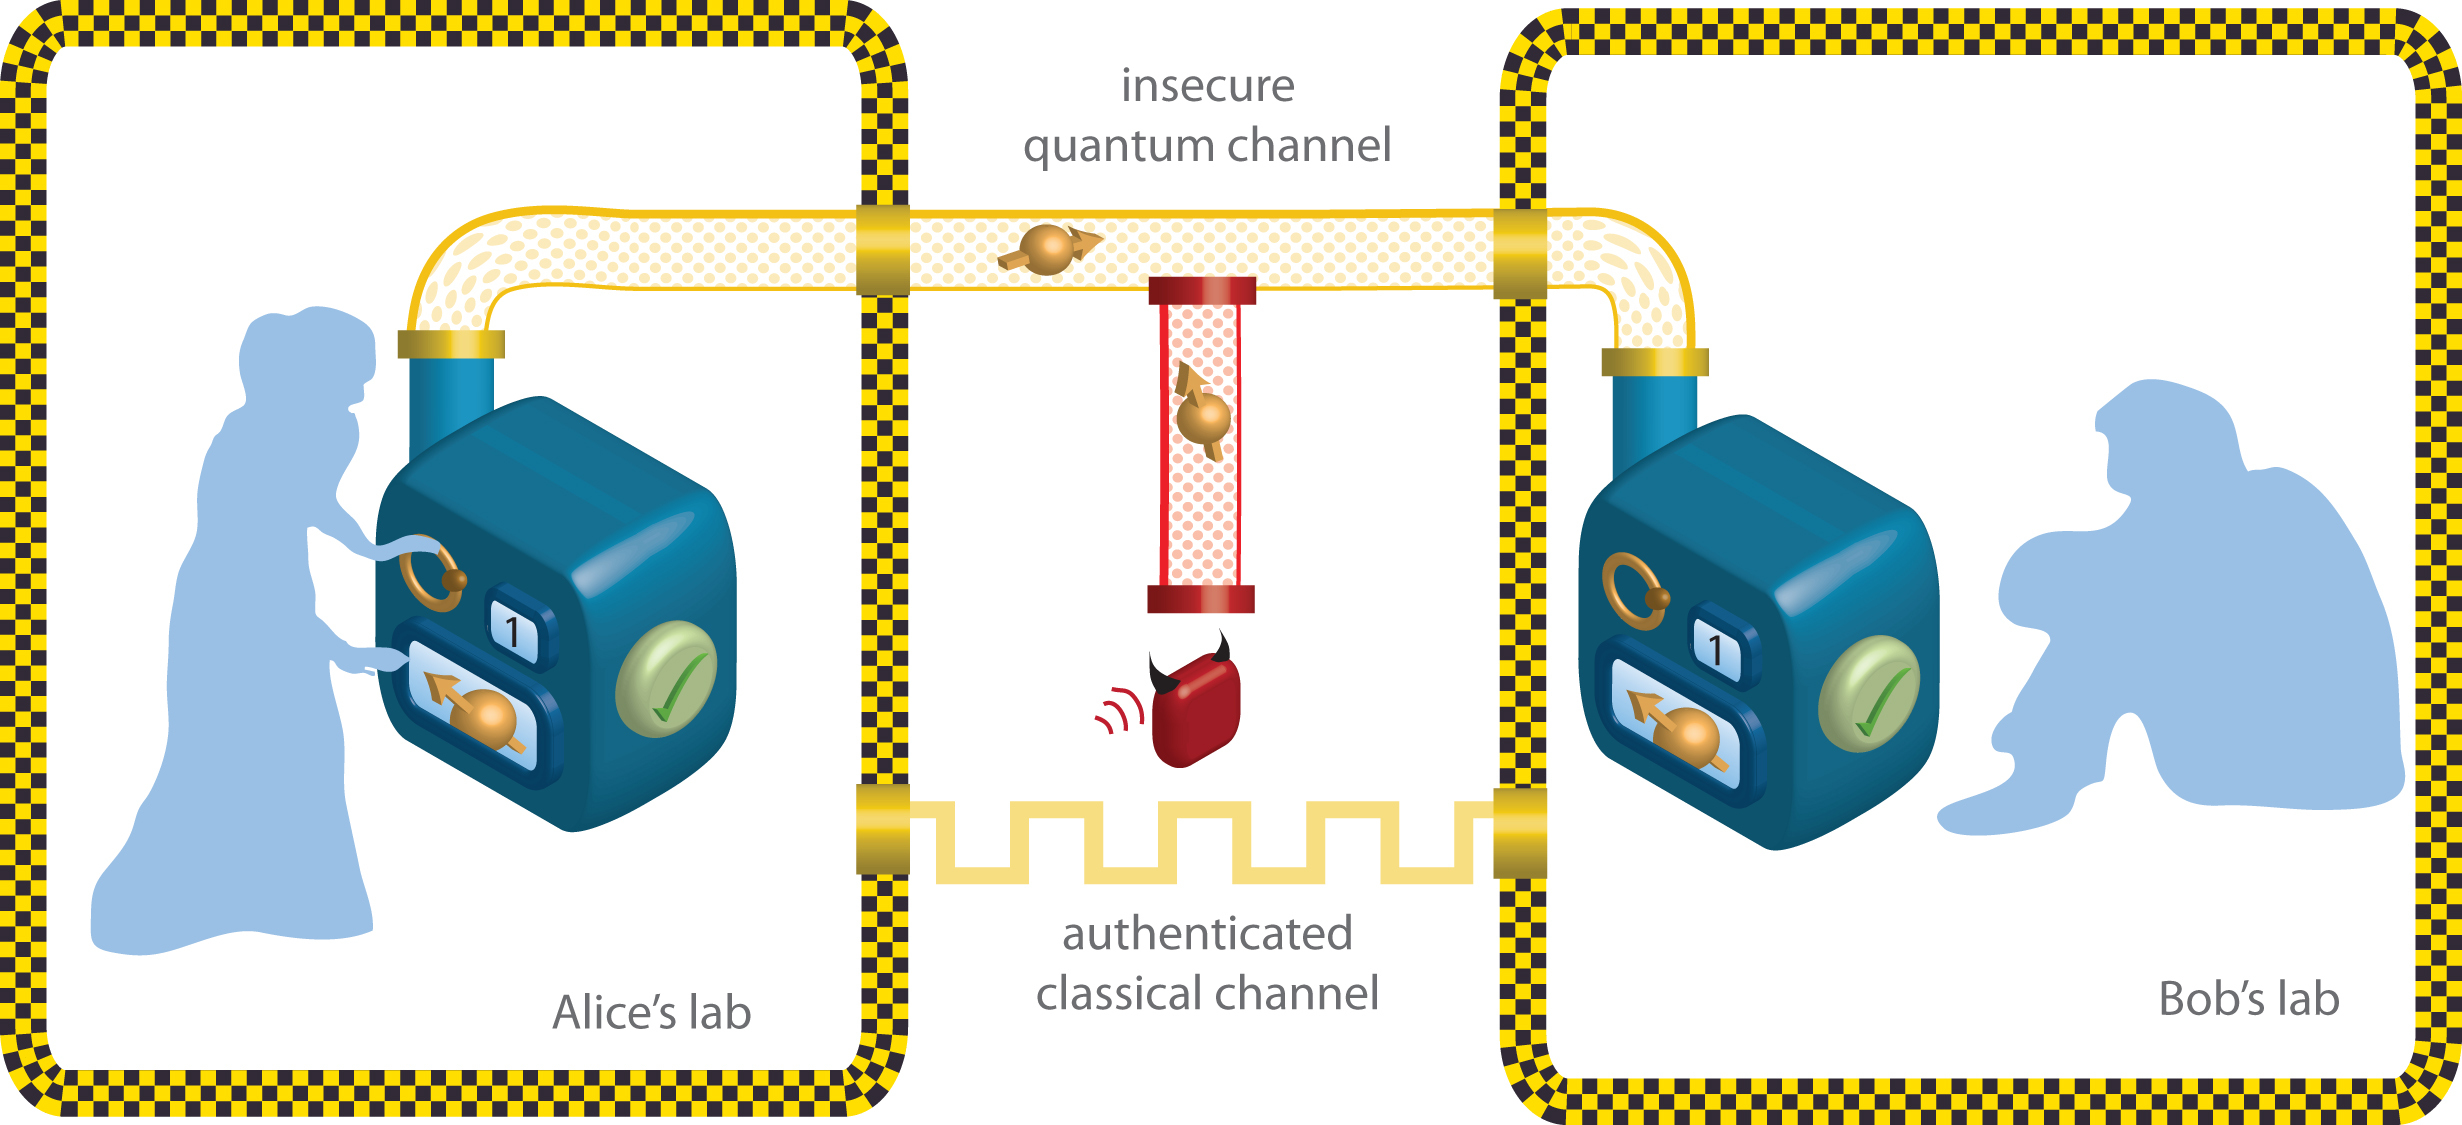
\includegraphics[trim={40px 80px 40px 25px},clip,width=0.9\textwidth]{quantum_alice_and_bob.jpg}
        \begin{itemize}
            \item $\left| \psi \right\rangle$ valamelyik bázis sajátvektora, de\\
                nem lehet tudni melyiké!
            \item Ha véletlen rossz bázisban mérünk, információt vesztünk.
            \item Módszer lehetne:
                \begin{itemize}
                    \item Lemásoljuk az állapotot.
                    \item Miután Alice és Bob megmondják bázisaikat, megmérjük azt.
                \end{itemize}
        \end{itemize}

    \end{frame}

    \subsection{Nemklónozhatósági tétel}

    \begin{frame}

        \center

        \textbf{Nemklónozhatósági tétel}

        \begin{itemize}
            \item Le lehet-e másolni kvantumállapotot?
            \item Többrészecskés kvantummechanika: tenzorszorzat tér.
            \item A másoló gép a következőt tegye:
        \end{itemize}

        \begin{equation}
            U: \left| \varphi \right\rangle \otimes \left| 0 \right\rangle
            \mapsto \left| \varphi \right\rangle \otimes \left| \varphi \right\rangle, \forall \left| \varphi \right\rangle
        \end{equation}

        \begin{itemize}
            \item Időfejlődés operátor unitér, ezért a gép unitér transzformációt végez.
            \item Bizonyítani lehet: nincs ilyen unitér transzformáció.
        \end{itemize}

    \end{frame}

    \subsection{Kvantum összefonódáson alapuló eljárások}

    \begin{frame}

        \center

        \textbf{Kvantum összefonódáson alapuló eljárás\\E91 protokol}

        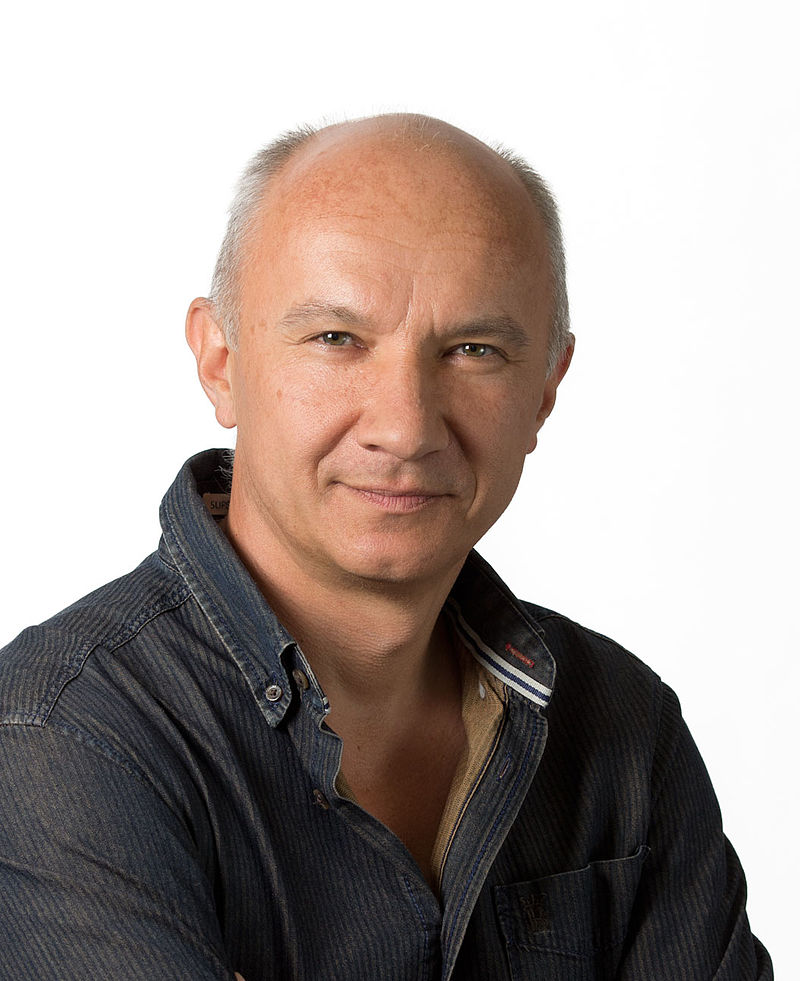
\includegraphics[height=100pt]{ekert.jpg}

        \begin{itemize}
            \item Artur Ekert, 1991
        \end{itemize}

    \end{frame}

    \begin{frame}

        \center

        \textbf{E91 protokol}

        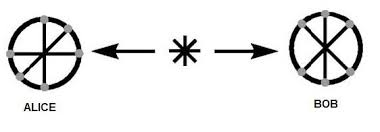
\includegraphics[width=0.3\textwidth]{e91source.jpg}

        \begin{itemize}
            \item Közös forrásból elektronokat küldünk Alicenak és Bobnak.
        \end{itemize}

        \begin{equation}
            \left| \psi \right\rangle =
            \frac{1}{\sqrt{2}} \left(
            \left| \uparrow \downarrow \right\rangle + \left| \downarrow \uparrow \right\rangle
            \right)
        \end{equation}

        \begin{itemize}
            \item Alice és Bob nem tudják előre mit fognak mérni, de tudják hogy a másik ellentétes spinvetületet mér, ha ugyanabban a bázisban mérünk.
            \item Legyenek bázisaink:\\
                $\phi^A_1 = 0 ^{\circ}, \phi^A_2 = 45 ^{\circ}\phi^A_3 = 90 ^{\circ}$
                $\phi^B_1 = 45 ^{\circ}, \phi^B_2 = 90 ^{\circ}\phi^B_3 = 135 ^{\circ}$
        \end{itemize}

    \end{frame}

    \begin{frame}

        \center

        \textbf{E91 protokol}

        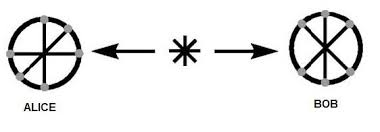
\includegraphics[width=0.3\textwidth]{e91source.jpg}

        \begin{itemize}
            \item Kulcskészítés:
                \begin{enumerate}
                    \item Véletlenszerűen választanak minden elektronspin mérésre egy bázist.
                    \item Mérések végén megosztják bázisaikat.
                    \item Ahol ugyanabban a bázisban mértek, az a kulcs értéke.
                \end{enumerate}
            \item 2/9 valószínűséggel választanak ugyanolyan bázist:
                \\az összes mérés 2/9-e lesz a teljes kulcs.
        \end{itemize}

    \end{frame}

    \begin{frame}

        \center

        \textbf{E91 protokol}

        \begin{itemize}
            \item Valaki megváltoztathatja Bob vagy Alice elektronjait.
            \item Így nem lesznek ugyanazok a kulcsok.
            \item Ellenőrzés:
                \begin{itemize}
                    \item Nem azonos bázisban mért elektronok korrelációját mérjük.
                    \item Ezek megoszthatók: nem a kulcs részei.
                    \item $E(a,b) = P_{++}(a,b) + P_{--}(a,b) + P_{+-}(a,b) + P_{-+}(a,b)$
                    \item $S = E(\phi^A_1, \phi^B_1)
                        - E(\phi^A_1, \phi^B_3)
                        + E(\phi^A_3, \phi^B_1)
                        + E(\phi^A_3, \phi^B_3)$
                    \item $S = 2 \sqrt{2}$, ha nincs lehallhatás (Bell egyenlőtlenségek).
                    \item $S \leq 2$, ha minden elektron lehallgatódott.
                \end{itemize}
            \item BB84 protokolban ahhoz, hogy megtudjuk jók-e a kulcsok meg kell azokat osztani részben.
        \end{itemize}

    \end{frame}

    \section{Kísérletek}

    \begin{frame}

        \center

        \textbf{Kísérletek:\\
            2008, Toshiba, University of Cambridge}

        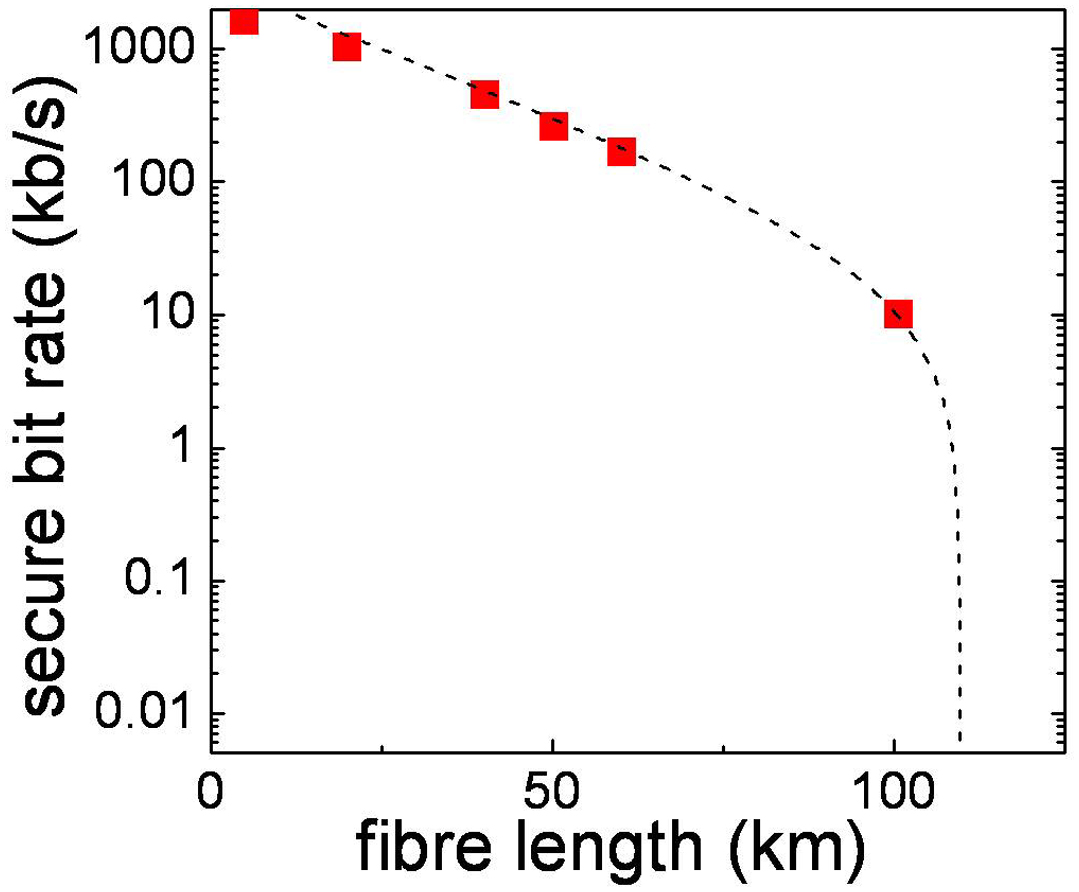
\includegraphics[height=100pt]{toshiba_exp_res.jpg}
        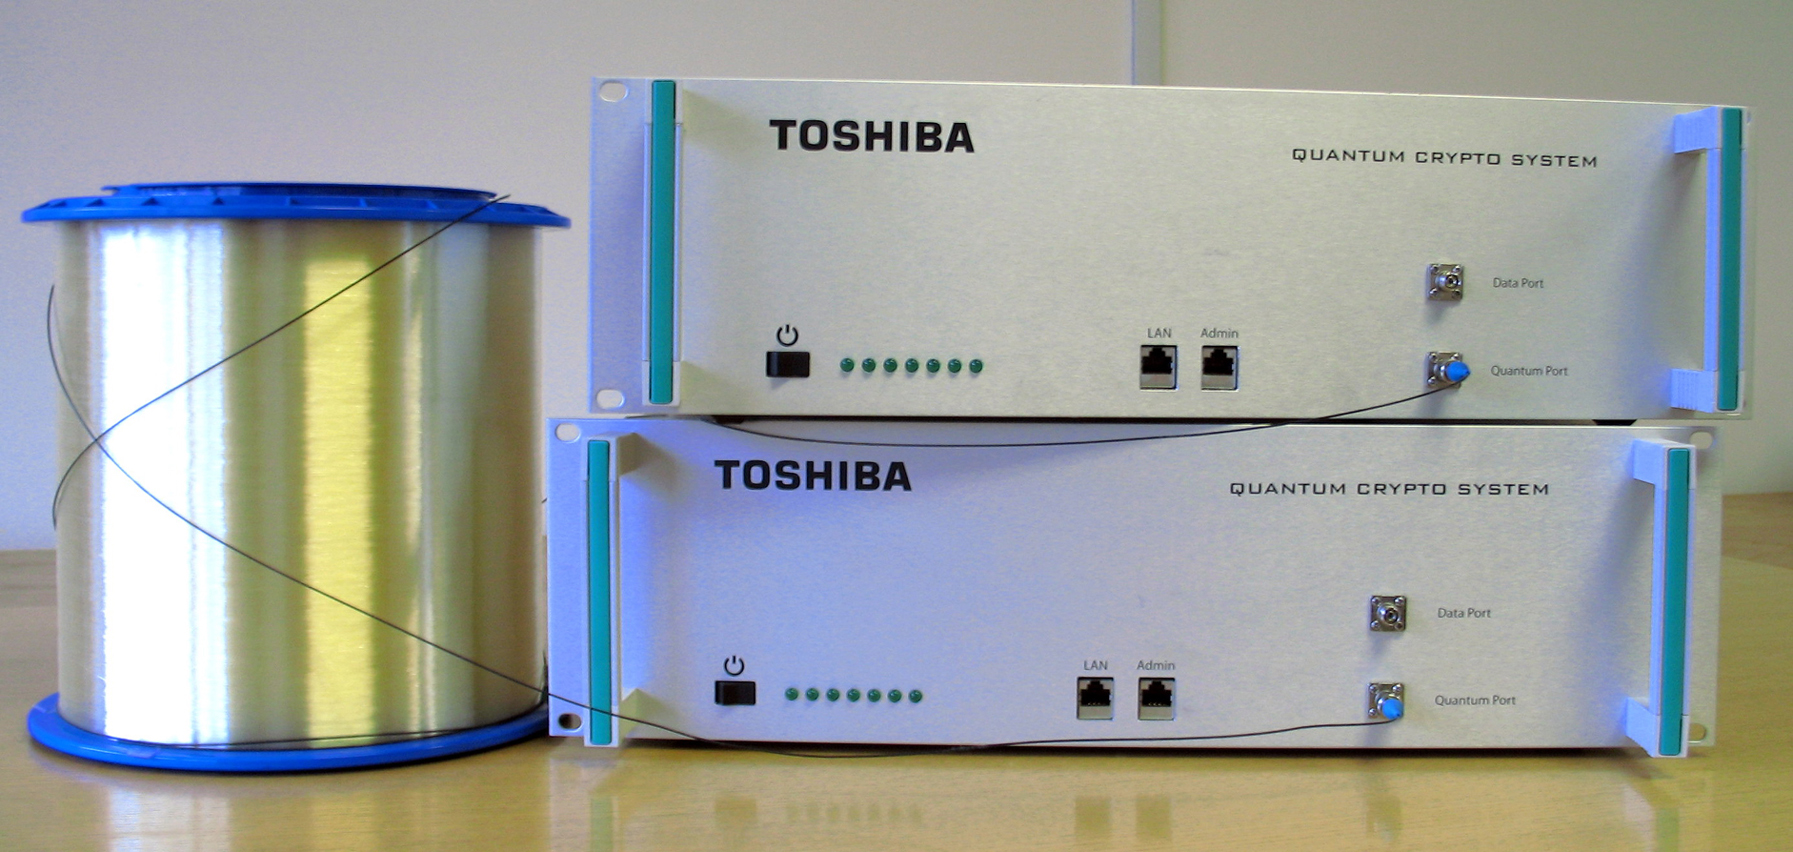
\includegraphics[height=100pt]{fiber.jpg}

        \begin{itemize}
            \item BB84 módosított változatát használták.
            \item Leggyorsabb adatátvitel titkos kulcsokra: 1 Mbit/s: 20 km optikai szálon, 10 kbit/s: 100 km-en.
            \item Fotonokat InGaAs Avalanche Photo Diode (APD) mérték\\
                Sok idő kell amíg újra használhatóak: nagy "dead-time",\\
                ez limitálja az adatsebességet.
        \end{itemize}

    \end{frame}

    \begin{frame}

        \center

        \textbf{Kísérletek:\\
            Kurtsiefer, 2002, A step towards global key distribution}

        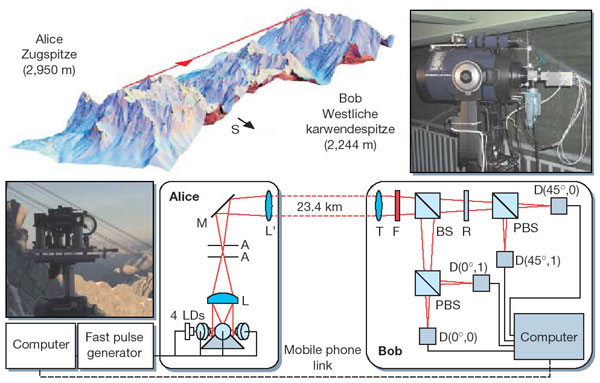
\includegraphics[width=0.8\textwidth]{austria_kurtsiefer.jpg}

        \begin{itemize}
            \item Ausztria, 23.4 km szabad optikai út
            \item BB84 módosított változata
        \end{itemize}

    \end{frame}

    \begin{frame}

        \center

        \textbf{Kísérletek:\\
            Kurtsiefer, 2002, A step towards global key distribution}

        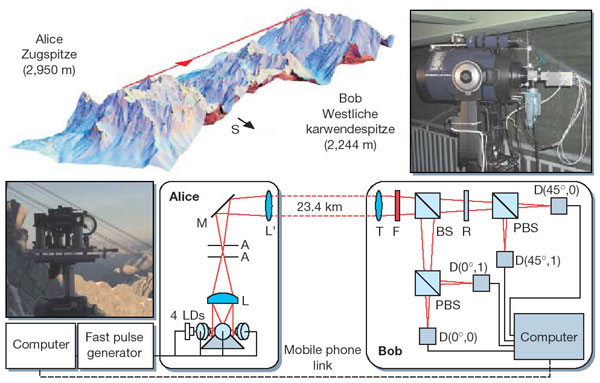
\includegraphics[width=0.8\textwidth]{austria_kurtsiefer.jpg}

        \begin{itemize}
            \item 18-20 dB veszteség
            \item 1.5-2 kbit/s
            \item Földközeli keringésű műhold kulcstovábbításhoz majdnem jó.
        \end{itemize}

    \end{frame}

    \begin{frame}

        \center

        \textbf{Kísérlet:\\
            Kanári szigeteki kvantum összefonodás kísérlet, 2006}

        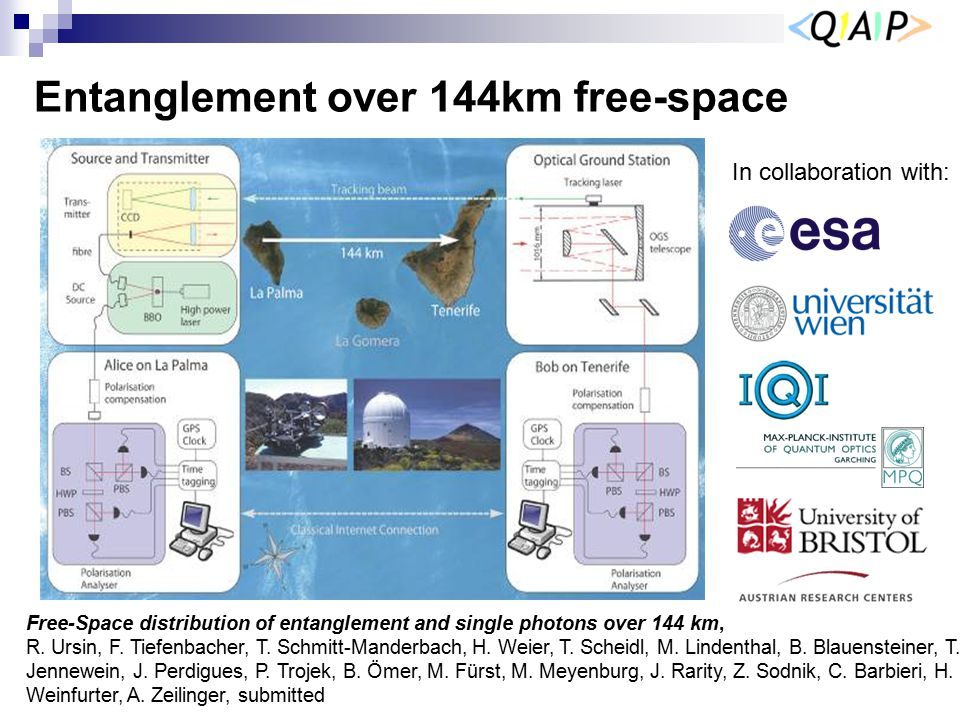
\includegraphics[width=0.8\textwidth]{canary_entanglement.jpg}

    \end{frame}

    \begin{frame}

        \center

        \textbf{Kísérlet:\\
            Kanári szigeteki kvantum összefonodás kísérlet, 2006}

        \begin{itemize}
            \item 144 km, szabad optikai út
            \item 355 nm hullámhosszú lézer
            \item Összefonódott fotonokat küldtek:
                $\frac{1}{\sqrt{2}}\left(\left| H \right\rangle_A \left| V \right\rangle_B - \left| V \right\rangle_A \left| H \right\rangle_B \right)$
            \item Beta Barium Borate (BBO) nemlineáris kristályt használtak.
        \end{itemize}

        
\includegraphics[width=0.8\textwidth]{bbo.png}

    \end{frame}

    \begin{frame}

        \center

        \textbf{Kísérlet:\\
            Kanári szigeteki kvantum összefonodás kísérlet, 2006}

        \begin{itemize}
            \item 75 s alatt 178 bites kulcsot küldtek.
            \item Mért $S \approx 2.508$ ($2 \sqrt{2} \approx 2.828$).
            \item kb. 30 dB veszteség
            \item Low Earth Orbit műholdak - Föld között kb. 1 nagysegrenddel nagyobb lenne a veszteség
        \end{itemize}

    \end{frame}

    \begin{frame}

        \center

        \textbf{Kísérlet:\\
            University of Geneva, 2015}

        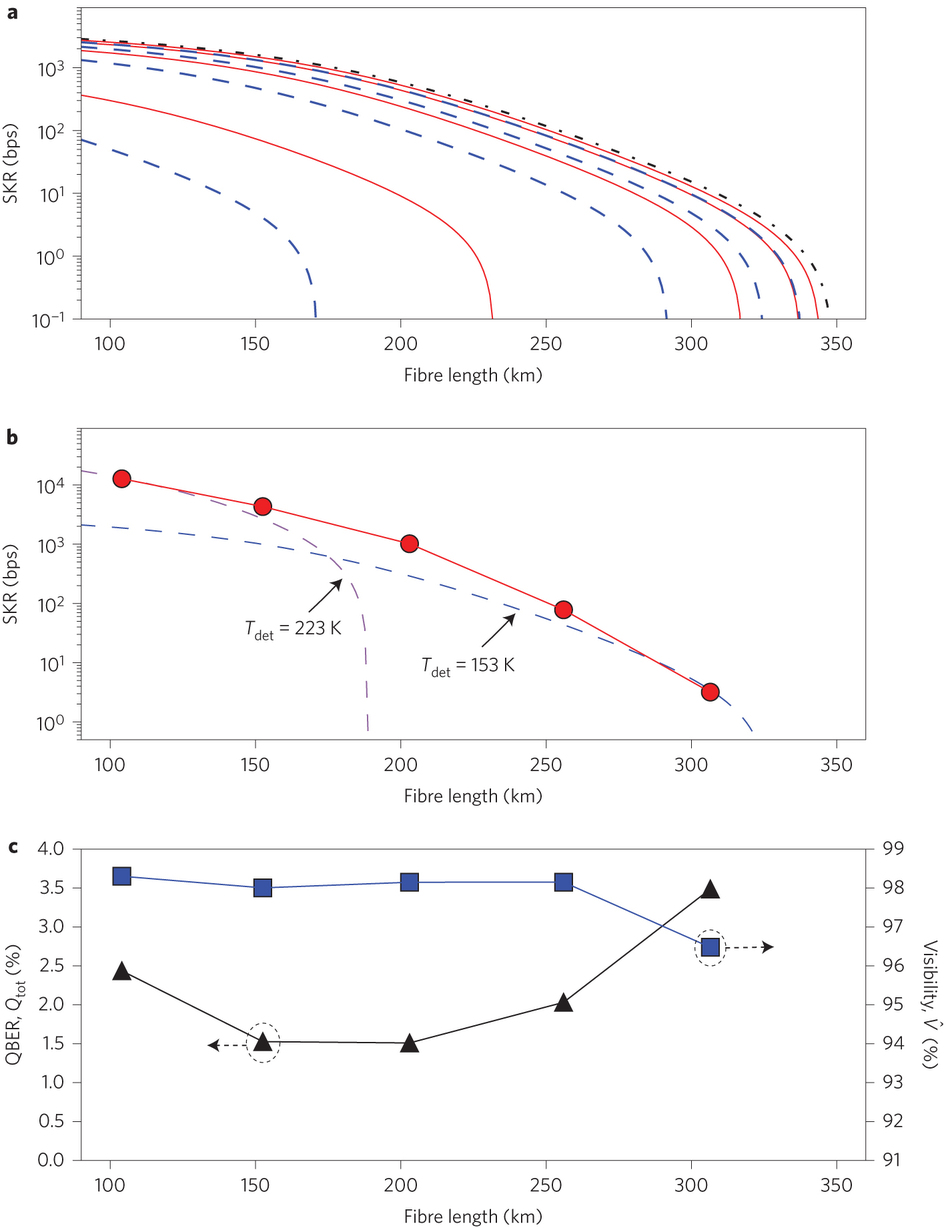
\includegraphics[trim={0 400px 0 400px},clip,width=0.9\textwidth]{geneva_bitrates.jpg}

        \begin{itemize}
            \item Leghosszabb út: 307 km, University of Geneva, 2015 (COW protokol).
            \item 307 km-en 3.2 kbit/s
        \end{itemize}

    \end{frame}

    \begin{frame}

        \center

        \textbf{Üzleti felhasználás}

        \begin{itemize}
            \item QKD-t nyújtó vállalatok: ID Quantique, MagicQ Technologies, QuintessenceLabs, SeQureNet
        \end{itemize}

        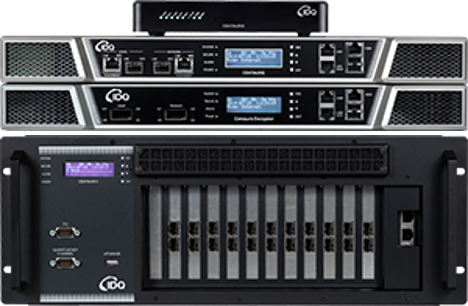
\includegraphics[width=0.4\textwidth]{idquantique.png}
        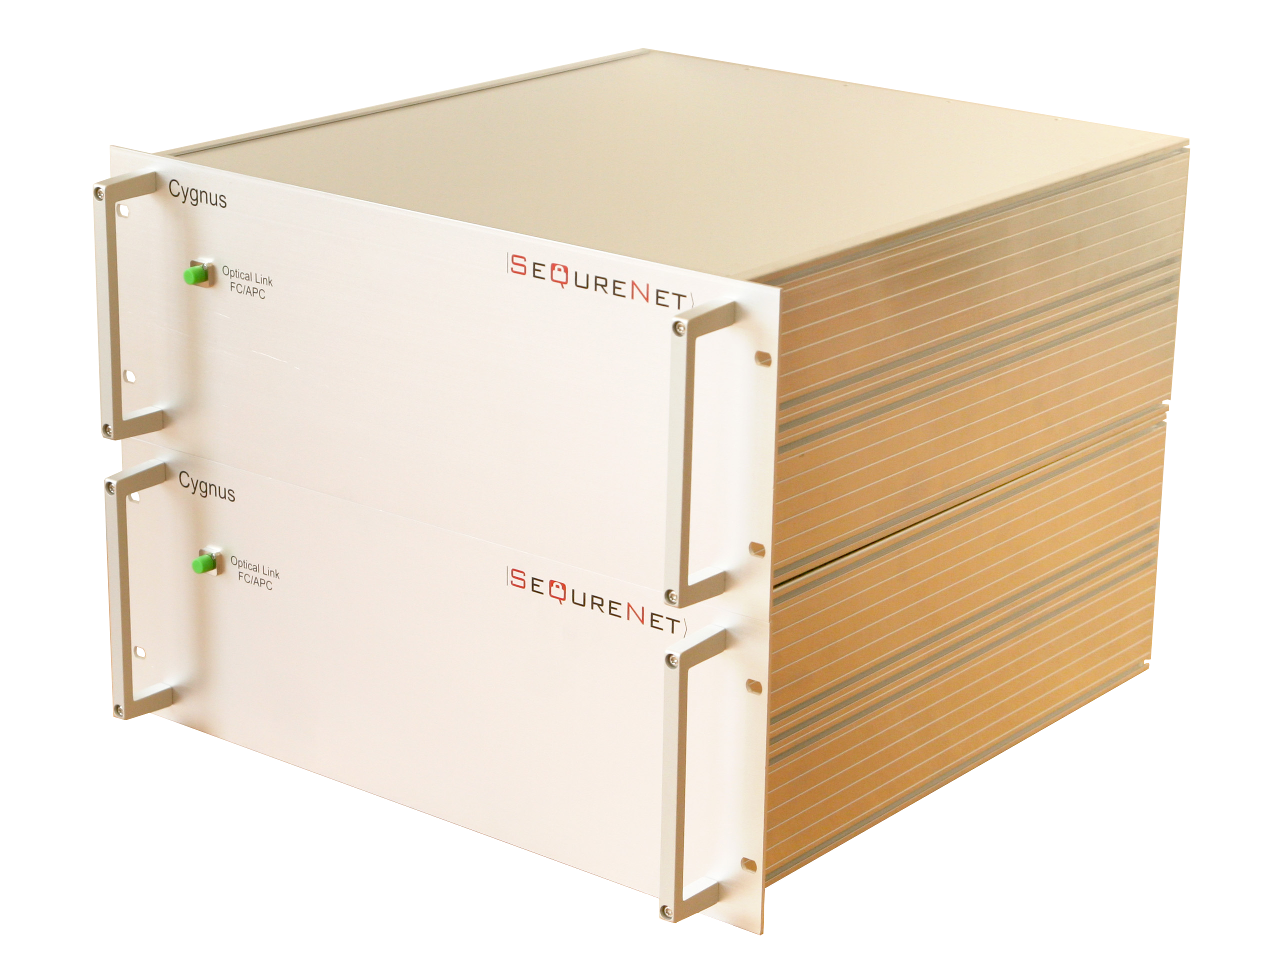
\includegraphics[width=0.4\textwidth]{cygnus_alice_bob.png}

        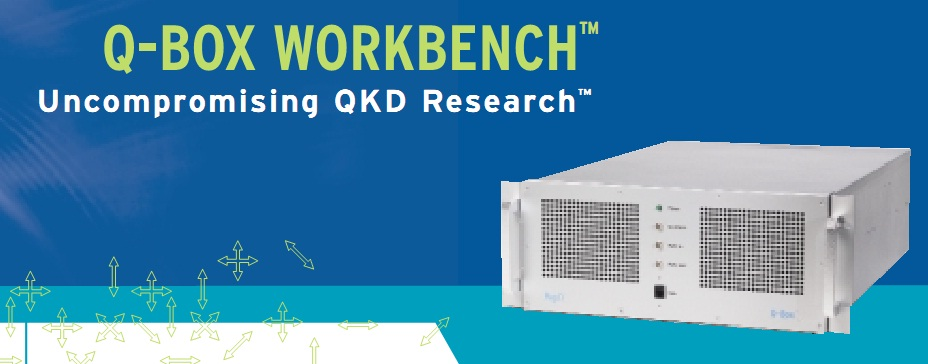
\includegraphics[width=0.6\textwidth]{qbox.jpg}

    \end{frame}

    \begin{frame}

        \center

        \textbf{Felhasználás}

        \begin{itemize}
            \item 2004, Bécs, első banki transzfer.
            \item 2007, Svájcban népszavazáshoz először használtak adatovábbításra
            \item DARPA 2004 óta 10 csomópontos quantum key distribution network
            \item Los Alamos Nation Laboratory: QKD network, de van központi hub
            \item 2008 óta EU Quantum Cryptography network: SECOQC (Secure Communication Based on Quantum Cryptography)
            \item Kvantum titkosított rendszerek ma még nagyon kevés helyen használatosak, ezek szinte mind kísérleti jellegűek.
        \end{itemize}

    \end{frame}

    \section{Források}

    \begin{frame}

        \center

        \textbf{Források}

        \tiny

        \begin{itemize}
            \item Bob és Alice grafika: \url{https://wordtothewise.com/2014/09/cryptography-alice-bob/}
            \item Diszkrét logaritmus eljárás: \url{https://en.wikipedia.org/wiki/Discrete_logarithm}
            \item RSA algoritmus: \url{https://en.wikipedia.org/wiki/RSA_\%28cryptosystem\%29}
            \item RSA-768 faktorizáció: \url{https://en.wikipedia.org/wiki/RSA_numbers\#RSA-768}
            \item Prímfaktorizáció kvantumszámítógéppel: \url{https://en.wikipedia.org/wiki/Shor\%27s_algorithm}
            \item Kvantumos Alice és Bob grafika: \url{http://www.proselex.net/Pages/SecretCommunication.aspx}
            \item QKD: \url{https://en.wikipedia.org/wiki/Quantum_key_distribution}
            \item BB84: \url{https://en.wikipedia.org/wiki/BB84}
            \item Benedikt Mihály jegyzete: \url{http://titan.physx.u-szeged.hu/~benedict/KvinfJ04.pdf}
            \item Bennet kép: \url{http://www.cs.bu.edu/new-CS-web/content/research/colloquium/10-Bennett.shtml}
            \item Brassard kép: \url{http://www.iro.umontreal.ca/~brassard/}
            \item Nemklónozhatósági tétel: \url{https://en.wikipedia.org/wiki/No-cloning_theorem}
            \item Artur Ekert: \url{https://en.wikipedia.org/wiki/Artur_Ekert}
            \item E91 protokol: \url{http://physweb.bgu.ac.il/COURSES/QuantumMechCohen/Contributions/yoav.pdf}
            \item E91 protokol: \url{http://www.ux1.eiu.edu/~nilic/Nina\%27s-article.pdf}
        \end{itemize}

    \end{frame}

    \begin{frame}

        \center

        \textbf{Források}

        \tiny

        \begin{itemize}
            \item Toshiba kísérlet: \url{http://spie.org/newsroom/technical-articles-archive/1519-record-quantum-cryptography-bit-rate-enables-ultrasecure-fiber-networks?ArticleID=x34398}
            \item Toshiba kísérlet arxiv: \url{http://arxiv.org/pdf/0810.1069.pdf}
            \item Kurtsiefert, A step towards global key distribution: \url{http://www.nature.com/nature/journal/v419/n6906/abs/419450a.html}
            \item Kurtsiefert, A step towards global key distribution: \url{http://xqp.physik.uni-muenchen.de/publications/files/articles\_2002/nature\_419\_450.pdf}
            \item Kanári szigeteki kísérlet: \url{http://lanl.arxiv.org/pdf/quant-ph/0607182v2}
            \item Spontaneous parametric down-conversion: \url{https://en.wikipedia.org/wiki/Spontaneous_parametric_down-conversion}
            \item BBO kristály: \url{http://nautil.us/issue/2/uncertainty/the-rise-of-the-uncertain}
            \item Leghosszabb QKD: \url{http://arxiv.org/pdf/1407.7427v1.pdf}
        \end{itemize}

    \end{frame}

    \section{}

    \begin{frame}
        \centering
        Vége.
    \end{frame}

\end{document}
